\subsection{UC32 - Visualizzazione errore tag non valido}
\begin{figure}[H]
  \centering
  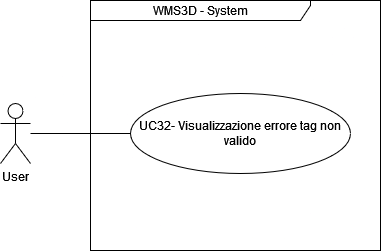
\includegraphics[width=0.5\textwidth]{UC_diagrams_28-32/UC32_sys.drawio.png}
  \caption{Diagramma UML UC32 - Visualizzazione errore tag non valido}
\end{figure}
\begin{itemize}
    \item \textbf{Attori:} User.
    \item \textbf{Pre-condizione:} Il tag della suddivisione inserito dall'utente contiene caratteri invalidi.
    \item \textbf{Post-condizione:} L'utente visualizza un messaggio d'errore e dovrà reinserire un tag diverso.
    \item \textbf{Scenario Principale:} L'utente visualizza un messaggio informativo sull'errore e ne conferma la ricezione. L'operazione fallisce e l'utente dovrà scegliere un nuovo tag.
    \item \textbf{Generalizzazioni:} -
    \item \textbf{Estensioni:} -
\end{itemize}